\documentclass[output=paper,colorlinks,citecolor=brown]{langscibook}
\ChapterDOI{10.5281/zenodo.15654881}
\title{\textit{Guth Thormoid}: The ``Island Voice" of Norman Maclean} 
\author{Gordon Wells\affiliation{University of the Highlands and Islands}}


\abstract{This chapter samples and contextualises some of the multi-faceted Gaelic contributions by the multi-talented creative icon, Norman Maclean, to the \textit{Guthan nan Eilean} `{Island Voices}' online language capture and curation project. These include, in particular, Norman's final \textit{Saoghal Thormoid} `Norman's World' series of videoed conversations, recorded in April 2016 in which he spoke reflectively of his memories and impressions of bilingual life in Glasgow and the Hebrides from the middle of the Twentieth Century onwards. In addition to offering a vivid first-person voiced and experiential account of Gaelic life over a tumultuous period for the language, the Island Voices adherence to basic linguistic principles pays dividends in relation to some initially unpredicted spin-off applications, with potential for further development.}


\IfFileExists{../localcommands.tex}{
   % add all extra packages you need to load to this file

\usepackage{tabularx,multicol}
\usepackage{url}
\urlstyle{same}

\usepackage{listings}
\lstset{basicstyle=\ttfamily,tabsize=2,breaklines=true}

\usepackage{langsci-basic}
\usepackage{langsci-optional}
\usepackage{langsci-lgr}
\usepackage{langsci-osl}
% \usepackage{./langsci/styles/langsci-lgr}
% \usepackage{./langsci/styles/langsci-osl}
% \usepackage{langsci-gb4e}

\usepackage{tikz}
\usetikzlibrary{patterns,calc}
\pgfdeclarepatternformonly{south east lines}{\pgfqpoint{-0pt}{-0pt}}{\pgfqpoint{3pt}{3pt}}{\pgfqpoint{3pt}{3pt}}{
    \pgfsetlinewidth{0.6pt}
    \pgfpathmoveto{\pgfqpoint{0pt}{3pt}}
    \pgfpathlineto{\pgfqpoint{3pt}{0pt}}
    \pgfpathmoveto{\pgfqpoint{.2pt}{-.2pt}}
    \pgfpathlineto{\pgfqpoint{-.2pt}{.2pt}}
    \pgfpathmoveto{\pgfqpoint{3.2pt}{2.8pt}}
    \pgfpathlineto{\pgfqpoint{2.8pt}{3.2pt}}
    \pgfusepath{stroke}}
    
\usepackage{stmaryrd}
\usepackage{wasysym}
\usepackage{multirow}
\usepackage{caption}
\usepackage{subcaption}
\usepackage{mathrsfs}
\usepackage{qtree}

\usepackage{linguex}


   %pminos do not split footnotes
% \interfootnotelinepenalty=10000 %Footnote in Laporte chapters has to be split SN


%\DeclareIndexNameFormat{default}{%
%\nameparts{#1}%
%\usebibmacro{index:name}%
%{\index[names]}%
%{\namepartfamily}%
%{\namepartgiveni}%
% {}% L1
% {}% L2
%{\namepartprefix}% generates spurious space L3
%{\namepartsuffix}% generates spurious space L4
%}

%  {\DeclareIndexNameFormat{default}{%
%     \usebibmacro{index:name}{\index[names]}{#1}{#3}{#5}{#7}}}

%\DeclareIndexNameFormat{default}{%
%  \usebibmacro{index:name}{\sindex[nom]}{#1}{#3}{#5}{#7}}

%\DeclareIndexNameFormat{default}{%
%  \usebibmacro{index:name}{\sindex[person]}{#1}{#3}{#5}{#7}}
%\DeclareIndexNameFormat{default}{%
%\nameparts{#1} \usebibmacro{index:name}{\sindex[person]]}{\namepartfamily}{‌​\namepartgiven}{\nam‌​epartprefix}{\namepa‌​rtsuffix}}

%\newcommand{\smiley}{:)}

%\renewbibmacro*{index:name}[5]{%
%\usebibmacro{index:entry}{#1}%
%{\iffieldundef{usera}{}{\thefield{usera}\actualoperator}\mkbibindexname{#2}{#3}{#4}{#5}}}

% \newcommand{\noop}[1]{}

%remove for final
%\overfullrule=1mm

\newcommand{\tobi}[2]}}
\renewcommand{\S}[1]{\tobi{#1}{\textsc{*}}}

% this volume references
% puts: [this volume]
% already defined: \citetv
%\newcommand{\citepv}[1]{(\citeauthor{#1} \citeyear*{#1} [this volume])}
\newcommand{\citealtv}[1]{\citeauthor{#1} \citeyear*{#1} [this volume]}

%parentheses around example number
\newcommand{\pref}[1]{(\ref{#1})}

% in-text examples

\newcommand{\lnex}[1]{\textit{#1}} %target lang word
\newcommand{\lnlit}[1]{(lit.: `#1')} %literal reading
\newcommand{\lnlat}[1]{(#1)} % latinization
\newcommand{\lntrans}[1]{`#1'} %translation
\newcommand{\lnexl}[2]%
{\lnex{#1}{} \lnlat{#2}} % ex with latinization
\newcommand{\lnexlat}[3]{\lnex{#1}{} \lnlat{#2}{} \lntrans{#3}} % ex with latinization and tranl.

%ch01
\newcommand{\co}[1]{\mbox{\textbf{#1}}}

%ch09

\newcommand{\cyrbulg}[1]{\begin{otherlanguage*}{bulgarian}#1\end{otherlanguage*}}


%ch10
\newcommand{\nlp}{{\small NLP}}
\newcommand{\mwe}{{\small MWE}}
\newcommand{\rae}{{\small RAE}}
\newcommand{\lvc}{{\small LVC}}
\newcommand{\pos}{{\small P}o{\small S}}
%\newcommand{\todo}[1]{ \textcolor{red}{#1} }

%\renewcommand{\labelenumi}{\theenumi}
%\ainamefmt{{vv}{ll}{, ff}{, jj}} % fullname

\newcommand{\biberror}[1]{{\color{red}#1}}

\newcommand{\osenovaitem}{--~}
   %% hyphenation points for line breaks
%% Normally, automatic hyphenation in LaTeX is very good
%% If a word is mis-hyphenated, add it to this file
%%
%% add information to TeX file before \begin{document} with:
%% %% hyphenation points for line breaks
%% Normally, automatic hyphenation in LaTeX is very good
%% If a word is mis-hyphenated, add it to this file
%%
%% add information to TeX file before \begin{document} with:
%% %% hyphenation points for line breaks
%% Normally, automatic hyphenation in LaTeX is very good
%% If a word is mis-hyphenated, add it to this file
%%
%% add information to TeX file before \begin{document} with:
%% \include{localhyphenation}
\hyphenation{
    Beck-man
    Ngu-yen
    back-chan-nel
    back-chan-nels
    mo-not-o-nous
    ste-reo-typ-i-cal
}

\hyphenation{
    Beck-man
    Ngu-yen
    back-chan-nel
    back-chan-nels
    mo-not-o-nous
    ste-reo-typ-i-cal
}

\hyphenation{
    Beck-man
    Ngu-yen
    back-chan-nel
    back-chan-nels
    mo-not-o-nous
    ste-reo-typ-i-cal
}

   \boolfalse{bookcompile}
   \togglepaper[13]%%chapternumber
}{}
\AffiliationsWithoutIndexing

\begin{document}
\maketitle

\il{Scottish Gaelic (Modern)|(}
\ia{Maclean, Norman|see {MacGill-Eain, Tormod}}
\ia{MacGill-Eain, Tormod|(}
\section{Introduction}

In this chapter, I describe the history and content of a documentation exercise focused on a singular individual, whose work emerged organically out of the Hebridean \textit{Guthan nan Eilean}\is{Guthan nan Eilean} `Island Voices\is{Island Voices|see {Guthan nan Eilean}}' language capture and curation project \citep{gw:Wells2023}. Specifically, it relates to the output of Norman Maclean, who was a person of many different talents and skills, and whose linguistic capacity was remarkable. As a case study, the approach is necessarily selective rather than comprehensive, seeking to give an indicative representation of Norman’s various contributions, though with a particular focus on his final recordings for the project.

I look at this output largely through applied linguistic eyes, with a fundamental orientation towards throwing light on the everyday Gaelic speech and culture of ordinary people. This may have the appearance of a somewhat paradoxical exercise. There is an inherent danger in attempting to draw widely applicable lessons from the study of \isi{exceptional exponents} of the language. Nevertheless, I hope to demonstrate that this exercise has delivered a valuable resource worthy of close study by anyone with an interest in contemporary vernacular Gaelic.

As a computer-mediated project with a focus on recorded Gaelic speech, its description through written English presents a challenge. However, numerous online links to recordings are given in footnotes.

I start with Norman’s self-introduction in \textit{Saoghal Thormoid}\is{Saoghal Thormoid} `Norman’s World,'\is{Norman's World|see {Saoghal Thormoid}} his final and weightiest contribution to Island Voices\is{Guthan nan Eilean}:

\begin{quote}
\textit{Tha fhios aig a h-uile Gàidheal cò e. M’ athair, ’s e Niall Mòr, mac Iain Eògh\-ainn Ruaidh à Cillmoluaig, Tiriodh. Maclean, a h-uile dàrna fear ann an Tir\-iodh ’s e Maclean a th’ orra. Ach sin mise air taobh m’ athar. An gille aig Niall Mòr, mac Iain Eòghainn Ruaidh. Air taobh mo mhàthar, mo mhàthair Peigi Bheag, nighean Anna Bige. Nis ’s e Anna Bheag a bha seo mo sheanmhair, ’s i nighean Aonghais ’ic Iain Mhòir à Hàcleit.} 
\end{quote}

\begin{quote}
`Every Gael knows who he is. My father, he’s Big Niall, son of Iain Eòghainn Ruaidh from Kilmaluaig, Tiree. Maclean, every second person on Tiree is a Maclean. But that’s me on my father’s side. Son of Big Niall, son of Iain Eòghainn Ruaidh. On my mother’s side, Wee Peggy, daughter of Wee Ann. Now my granny Wee Ann, she’s the daughter of Angus, son of Big Iain from Hacklett.' (Tormod MacGill-Eain)\footnote{\url{https://youtu.be/nCR2mVnDcX0}} 
\end{quote}

This can be taken as an example of a once typical Gaelic personal introduction, through the subject’s \textit{sloinneadh}\is{sloinneadh}, or genealogy\is{genealogy|see {sloinneadh}}. It is a traditional naming system which relies largely on patronymics, though matronymics may also be used. In fact, in this case we’re given both sides of Norman’s family. 

By way of my own self-introduction, I also have a \textit{sloinneadh}\is{sloinneadh}: \textit{Is mi an gille as òige aig Anna Sheonaidh ’ic Ghilleasbaig} `I’m the youngest son of Anna, daughter of Seonaidh, son of Gilleasbaig.’ It is an important introductory point to make that this is how people in the North Uist community into which my mother was born know themselves and know each other. This is how you identify friends, relations, and other community members. In other terms it might be so said to help present or mediate, at least to some extent, my own ``positionality” \citep{gw:Greenbank2003} 
with respect to the community. 

That being said, I was actually born in Edinburgh and raised speaking mostly English, firstly for a short while in India, then in England, and did not ``come home” to live in Uist until my fortieth year. In this respect, my perspective on the islands community in which I then became a resident remains in part an external one, complemented by an academic background in Linguistics and Applied Linguistics, and a professional training and working experience as a language teacher and researcher. 

The \textit{Guth Thormoid} in the title of this article translates as `Norman’s Voice’. The “Island Voice” element is placed in quotation marks for emphasis, because Norman had many voices, and they weren’t all island ones by any means. However, this article concentrates on his contributions to the above-mentioned Island Voices\is{Guthan nan Eilean} or \textit{Guthan nan Eilean}\is{Guthan nan Eilean} project, which I co-ordinate.

\is{Guthan nan Eilean|(}
The rest of this article gives further information about Norman, about the Island Voices project, and about his contributions to it. Attention is paid to his \textit{Saoghal Thormoid}\is{Saoghal Thormoid} series of conversations. Following this, a brief description is given of some spin-off applications, which were quite unpredicted at the outset of the work, but which can be seen as natural progressions out of the fundamentally linguistic orientation of the project at its inception. The article concludes with some summary points on Norman’s special contribution to the Island Voices project.
\is{Guthan nan Eilean|)}

\section{Norman Maclean}

\begin{figure}[t]
    \includegraphics[width=\textwidth]{figures/Wells-img002.png}
    \caption{\textit{Dìleab Thormoid} `Norman’s Legacy' screenshot: \url{https://guthan.wordpress.com/2017/09/18/dileab-thormoid-dhuinn/}}
    \label{fig:wells:1}
\end{figure}

Many appreciations have been written about the multi\hyp talented and multi\hyp lingual Norman Maclean (26 December 1936–31 August 2017), or \textit{Tormod MacGill-Eain} as he was known in Gaelic. His creative work was wide-ranging across various genres, with notable success as a comedian, novelist, poet, piper, singer, actor and broadcaster. He famously won both Bardic Crown and Gold Medal at the same Royal National Mòd in 1967. Born in Glasgow to Hebridean parents (from North Uist and Tiree), he was raised in various Gaelic-speaking households in the city itself, as well as Lochaber and then Benbecula when evacuated as a child during the war period. He struggled openly with alcoholism for many years, but he found some peace on retiring to Uist for the final decade or so of his life. His was a well-known and well-loved name in the Gaelic world.

\is{Guthan nan Eilean|(}
My own personal acquaintance with him was limited. I did not get to know him until he had entered his eighth decade. But I’m happy to vouch for his talent, which I was pleased to witness on various occasions, and for his generosity, particularly with his time, given the signal contribution he made in various ways to the Island Voices project itself. So when he passed we did write our own tribute (see \figref{fig:wells:1}). It is written in Gaelic, but the top paragraph actually links through to a number of obituaries which were published in national and local press as well as online, so further information on his life and times is readily available in English through the Island Voices site.
\is{Guthan nan Eilean|)}


\section{Island Voices}

\is{Guthan nan Eilean|(}

\begin{figure}[ht]
    \includegraphics[width=\textwidth]{figures/Wells-img001.png}
    \caption{About Island Voices Screenshot: \url{https://guthan.wordpress.com/about/}}
    \label{fig:wells:2}
\end{figure}

Island Voices has a presence in various corners of the Internet, (principally on \url{http://WordPress.com} and \url{http://youtube.com}). It also has social media channels through Twitter and Facebook. The project is conceived as a ``language capture and curation project.” We record linguistic material, and we display it. The approach has been bilingual from the start. It is now multilingual, but Gaelic has a central role given the Hebridean locus and focus of the project. It is all online, and there’s free and open access across the world~-- not just in the islands which are the geographical centre of interest. We’re open to everybody.

The project has gone through various phases, starting in 2005 and going online three or four years after that. Initially, the orientation was towards pedagogical development in terms of language learning and teaching~-- looking at methods and methodologies, and technologies. That was a staff-led period, in which project staff~-- principally myself~-- produced short documentaries to focus on a particular topic or venue in the community, and complemented those with authentic speech \citep{gw:Widdowson1998} 
talking-head interviews with local members of the community who had a particular connection with that topic.

After establishing a central core of materials (Series One and Two), we moved on from the initial staff-led approach to something more participatory, encouraging local community members and local community groups to initiate the same kind of work – to collect or create recordings and then share them through our Island Voices websites. And that continues to be the ethos as we go on. The tabs at the top of \figref{fig:wells:2} 
illustrate how over the years we’ve created a good number of different pages, which show the topical range of the full Island Voices project. A page basically consists of one or two tables, and each table contains multiple links to materials which we’ve produced in various formats. Among the collection of pages on the site there is a dedicated `Norman Maclean' one, in light of the significant amount of material which he himself produced.

The first 150 videos were created in the staff-led phase referred to above. These are the more pedagogically oriented materials in Series One and Series Two Outdoors, Generations, and Enterprise. Since then, with the broadening out of the focus and participation, we’ve more than doubled the number of videos which we have on the YouTube site. And the orientation itself has widened from a focus on language learning and language teaching to welcome participation across the community, including in particular from people to whom Gaelic proficiency and habitual use have come as an unremarkable and natural function of being raised in a Hebridean home.

Of course, we’re pleased if we can continue to help people learn the language. We think that we can help them do that through profiling unmarked, functional language in use.

\begin{figure}[ht]
% % %     \includegraphics[width=.4\textwidth]{figures/Wells-img003a.png}
% % %     \includegraphics[width=.4\textwidth]{figures/Wells-img003b.png}
% % %     \includegraphics[width=.4\textwidth]{figures/Wells-img003c.png}
% % %     \includegraphics[width=.4\textwidth]{figures/Wells-img003d.png}
    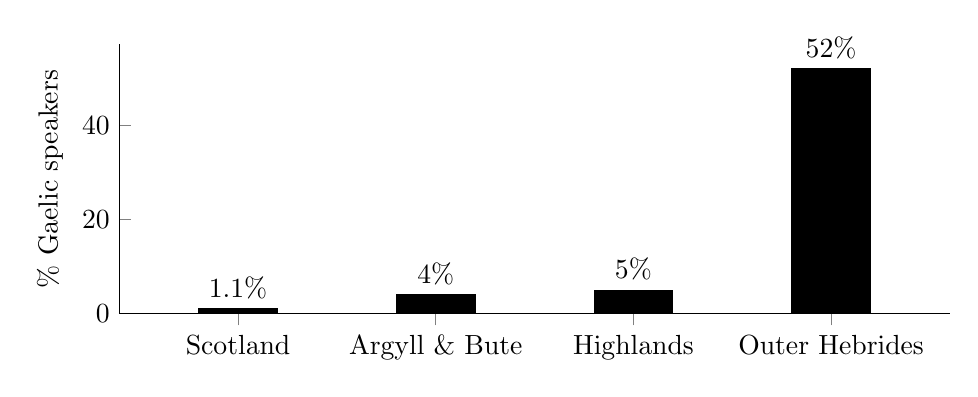
\begin{tikzpicture}
      \begin{axis}[ybar,
                   axis lines*=left,
                   symbolic x coords = {Scotland,Argyll \& Bute,Highlands,Outer Hebrides},
                   xtick = data,
                   width=\textwidth,
                   height=5cm,
                   bar width=1cm,
                   enlarge x limits = 0.2,
                   nodes near coords=\pgfmathprintnumber{\pgfplotspointmeta}\%,
                   ylabel = {\% Gaelic speakers},
                   ylabel near ticks,
                   ymin=0
                  ]
      \addplot [fill=black,draw=black] 
                coordinates {
                              (Scotland,1.1) 
                              ({Argyll \& Bute},4)
                              (Highlands,5)
                              (Outer Hebrides,52)
                            };
      \end{axis}
    \end{tikzpicture}
    \caption{2011 Census returns on Gaelic speaker percentages \citep{gw:Scotland’sCensus2011}}
    \label{fig:wells:3}
\end{figure}

The project title “Island Voices” has two elements. Census returns from 2011 explain the significance of the `Islands' element in relation to Gaelic. It is worth noting that the bar charts in \figref{fig:wells:3}, based on the 2011 census, rely on self-report data from questions asked across Scotland about speaking Gaelic \citep{gw:Scotland’sCensus2011}. Even with this caveat, they give a clear indication that of the various local authorities it is only in the Outer Hebrides that such a significant proportion of the population is found speaking Gaelic, or at least claiming to speak it. It dwarfs the figure for the proportion of the total population of Scotland. So there is clearly a special connection between Gaelic and these islands.\footnote{\citet{gw:ÓGiollagáin2020} offer fine-grained analysis to suggest a figure of 11,000 vernacular speakers of Gaelic in their islands study area.}

\begin{figure}[ht]
% % %     \includegraphics[height=.35\textheight]{figures/Wells-img004.png}
    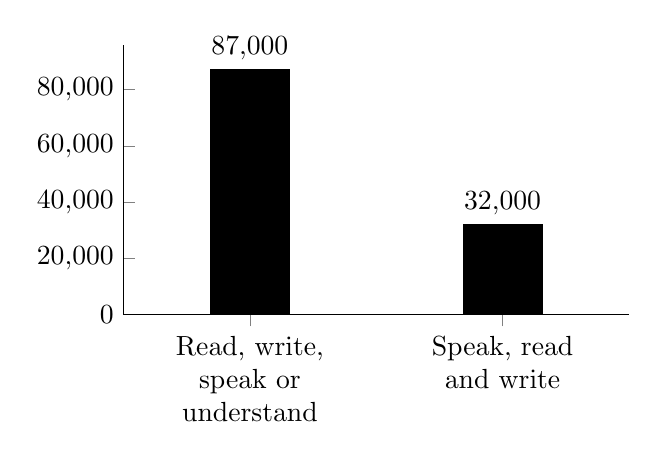
\begin{tikzpicture}
      \begin{axis}[ybar,
                   axis lines*=left,
                   symbolic x coords = {{Read, write, speak or understand},{Speak, read and write}},
                   xtick = data,
                   x tick label style={align=center, text width=2.5cm},
                   enlarge x limits = 0.5,
                   scaled y ticks=false,
                   width=8cm,
                   height=5cm,
                   nodes near coords, 
                   bar width=1cm,
                   ymin=0
                  ]
      \addplot [fill=black,draw=black] 
                coordinates {
                              ({Read, write, speak or understand},87000) 
                              ({Speak, read and write},32000)
                            };
      \end{axis}
    \end{tikzpicture}
    \caption{Census figures on Gaelic reading, writing, and speaking skills \citep{gw:Scotland’sCensus2011}}
    \label{fig:wells:4}
\end{figure}

\largerpage
Census figures, as shown in \figref{fig:wells:4}, 
on Gaelic reading, writing, and speaking skills also underline the significance of the ``Voices" element in the project title. There is a clear discrepancy between the number of people who speak the language and the number who read and write it as well. Island Voices is about oracy, and the primacy of speech 
(\citealt{gw:Sapir1921}, \citealt{gw:Bloomfield1933}, \citealt{gw:deSaussure1966}, \citealt{gw:ChafeTannen1987}, \citealt{gw:Wells2020}). 
That is what we want to address and profile particularly. It is a distinguishing feature of the overall picture that the best speakers of Gaelic, being the people who have been brought up using it, have not necessarily received an education through it. They are certainly literate, but their trained literacy is in their other language. We should not let them feel that their Gaelic skills are not recognised or valued simply because they do not read or write it. We need to actively profile the spoken language, and that is what Island Voices undertakes to do as a primary goal.
\is{Guthan nan Eilean|)}

\section{Norman Maclean and Island Voices}

\is{Guthan nan Eilean|(}

\figref{fig:wells:5} collects a number of screenshots that trace the history of Norman’s involvement with Island Voices. ``Island Voices Enterprise” is an example from the staff-led beginnings of the project, where we had topics that were introduced in staff-produced short documentaries, complemented with talking head interviews with people associated with the topic. Below this, the table from the Island Voices Enterprise page tab shows the bilingual presentation – English on the left, Gaelic on the right – with a short documentary on the \textit{Am Pàipear} community newspaper in plainer ``teacher talk” language, followed by the personal interviews, which are the interesting part from the point of view of recorded authentic speech. Tormod MacGill-Eain, or Norman Maclean, is listed amongst these. This dates from 2010.
 
 \begin{figure}
    \includegraphics[width=\textwidth]{figures/Wells-img005.png}
    \caption{Norman and Island Voices Screenshot Collage (click on link for larger image): \url{https://guthan.files.wordpress.com/2023/06/tormod-slide-8.pdf}} 
    \label{fig:wells:5}
\end{figure}

In the middle section of \figref{fig:wells:5}, we move into more participatory work involving local individuals and groups. As an example, we created a page called Storytellers, because one of our Island Voices activists, Mary Morrison, was keen to go out into the community and record people telling stories. We have two of Norman’s stories at the top of that table. This moves us into a different functional genre – that of narration. The second example in the central column is from our Great War project, which was led by the North Uist Historical Society in 2014, marking the 100\textsuperscript{th} anniversary of the outbreak of World War One. Local society members made recordings in the community. One of these was a video of Norman reciting one of his own poetic compositions to local schoolchildren in the Carinish School where his mother had been a pupil.

On the right of \figref{fig:wells:5} is Norman Maclean’s own dedicated page. It has two parts to it – Number Two, \textit{Sgeulachdan Thormoid}, and Number One, \textit{Saoghal Thormoid}\is{Saoghal Thormoid}. \textit{Sgeulachdan} means ‘stories’. This was his initiative. He came to us, and although it is listed as Number Two, it was in fact the first of these two parts chronologically. Norman wanted to record some of his short stories which he had been writing for the benefit essentially of young people who might want to get up on stage and perform a recitation in a local competition or even at the National Mòd. He was keen to get these recorded and available for people to view, so we were more than happy to accommodate his wish.

\is{Saoghal Thormoid|(}
That sparked \textit{Saoghal Thormoid} very soon thereafter when the then director of Soillse, Professor Conchúr Ó Giollagáin, spotted \textit{Sgeulachdan} and suggested we follow it up with some discursive recordings in which Norman would be encouraged to look back on his long and interesting life. Luckily, Norman was happy to oblige, and I was given the privilege of going into his house on consecutive days for a full week, just to let him speak and to record his words. This substantial and significant \textit{Saoghal Thormoid} collection was Norman’s last contribution to Island Voices. The videos were placed online with \isi{Clilstore} transcriptions (see \sectref{sec:wells:clilstoreDASG} below) on completion in November 2016. A printable volume was later uploaded \citep{gw:Wells2017}, including a foreword from Ó Giollagáin concluding with this summation (p4): ``Tormod’s life is an acknowledgement of the cultural wealth of Gaelic society, and by virtue of this archive, he represents an ambassador to its future.”
\is{Saoghal Thormoid|)}

The following account gives a summary description of each day’s conversation supplemented with brief commentary and selected quotes to highlight points of particular interest. 

\is{Guthan nan Eilean|)}

\section{Saoghal Thormoid: Norman’s world}

\is{Saoghal Thormoid|(}

\subsection{Monday: Ancestry}

\textbf{Summary}:``Every Gael knows who he is.” Norman talks about his genealogy\is{sloinneadh}, on both sides of the family, and how these family networks played an important part in his early upbringing in Glasgow, Lochaber, and Benbecula. He has clear memories of his paternal grandfather teaching him songs, a man who himself won a prize for Gaelic singing at the Falkirk Tryst of 1878. His maternal grandmother, meanwhile, migrated to Glasgow from North Uist and never learned to speak English, functioning socially just within the Gaelic-speaking community of Glasgow of that time. Norman reflects on how community relations were experienced from different perspectives in his childhood.

\is{sloinneadh|(}
In giving Norman’s \textit{sloinneadh} in the introduction to this article, I’ve already quoted from this conversation. But in addition to the importance of the \textit{sloinneadh} (which might contain other elements beyond the purely genealogical – for example physical attributes, such as \textit{Niall Mòr} – ‘Big Neil’, or \textit{Peigi Bheag} – ‘Wee Peggy’), the reference to Gaelic signals a key theme, and the introduction of social commentary, right from the start, is also noteworthy. It recurs throughout all five days of the conversations. He was constantly contextualising what he was telling us, by explaining what was happening around him at the time, as this extract illustrates:
\is{sloinneadh|)}

\begin{quote}
``\textit{… Ach, ’s e cailleach smart a bh’ innte}. But, \textit{thuirt mo mhàthair, an uair ud ann an Glaschu, cha ruigeadh i leas Beurla a bhith aice. Bha uiread de Ghàidheil timcheall oirre, agus bhiodh i – daoine a’ bruidhinn mu dheidhinn} Muslim isolation\textit{is gnothaichean – cha do rinn i oidhirp sam bith Beurla ionnsachadh. Bha nighean aice a sgrìobhadh litrichean dhi – seo mo mhàthair. Chan e gur e} Nobel prize-winner\textit{a bha nam mhàthair, ach, }you know\textit{, bha comas sgrìobhaidh aice. Bhiodh ise a’ sgrìobhadh. Bha na gillean, Tormod is Seumas is Cailean – rachadh iadsan dha na bùithtean dhi airson biadh, agus, recreation mar a chanas iad, well rachadh i a thaigh a’ Bharraich air }Paisley Road…" 
\end{quote}

\begin{quote}
`… But she was a smart old woman. But, my mother said, at that time she didn’t need English. There were so many Gaels around her, and she would – people talking about Muslim isolation and things – she made no effort to learn English. She had a daughter who would write letters for her – this is my mother. Not that my mother was a Nobel prize-winner, you know, but she could write. She would write. The boys, Tormod and Seumas and Cailean – they would go to the shops for her for food, and, recreation as they say, well she would go to the Barrach’s house on Paisley Road…' (Tormod MacGill-Eain) \footnote{\url{https://youtu.be/nCR2mVnDcX0}} 
\end{quote}

\noindent{Here Norman talks about his grandmother and explains about her Gaelic and English language skills and practices in a description which might equally fit numerous other migrant community circumstances. She did not speak any English as she did not need to. She had children who’d look after everyday communicative needs. And if she needed entertainment she would go and visit other Gaels in Glasgow.}

So he keeps a running social commentary, and it is not just about then, but it is also about now, with the parenthetical reference to so-called ``Muslim isolation”. This recording was made in 2016 around the time when a national report \citep{gw:Casey2016} 
was in the news, which affected to be concerned about community integration in the UK, and expressed some worries about levels of English language skills amongst certain communities. Norman clearly had no truck with the apparent controversy. It did not impress him at all that it was considered to be a matter of some concern that when people moved in a community to a new place they continued speaking their own language, particularly if they had other people from their own community around them. He had seen something very similar before in his own family history, and so made the link to contemporary life.

\subsection{Tuesday: Education}

\textbf{Summary}: After offering some further thoughts on the dominant Catholic/Pro\-tes\-tant divide in the Glasgow of his youth, Norman goes on to trace his educational journey, with customary vivid detail and illustrative anecdote, through primary schools in Lochaber, Benbecula and Glasgow, and on to Bellahouston Academy and Glasgow University. He discusses the constraints on, and the opportunities for, varied language choices he and others made in these contexts, within and outwith home and school environments, reflecting also on the Gàidh\-eal\is{Gàidheal}-\isi{Gall} relationship in Glasgow, and some of the wider educational choices he made at that time.

On Tuesday, when Norman describes his journey through education, significantly it is a history not confined to Glasgow. It also includes other schools in the Highlands and in Benbecula during the war period when he was evacuated out of the big city. It is worth noting in passing that this account is full of rattling yarns, narrated in his own unique style. Creamola crops up. So does Louis d’or. The broader point here is that community relations are figuring again. He talks about Glasgow and the very dominant and obvious Catholic/Protestant divide as it was felt in the part where he lived, and the relationship between \textit{Gàidheal}\is{Gàidheal} and \textit{Gall}\is{Gall}, between Gaelic speaker and non-Gaelic speaker. These were salient points for him as he was progressing through his education.

\begin{quote}
\textit{Ach nach eil e neònach mar a bha m’ inntinn ag obair nuair a bha mi beag. Nuair a bha mi còmhla ri muinntir Ghlaschu, còmhla ris a’ chloinn, cha robh ann ach dà roghainn san t-saoghal. Cha robh ann ach dà threubh – Pròstanaich is Caitligich. Agus cha robh iad a’ tighinn ri chèile uair sam bith. Nis, nach eil e neònach, leis a’ chloinn aig an robh pàrantan às Uibhist a Deas, ’s à Èirisgeigh ’s à Barraigh, Caitligich, cha robh dad sam bith, cha robh cnap-starra sam bith eadar an dà threubh, ach le muinntir Ghlaschu bha e cho soilleir, bha e dìreach ann an dubh ’s an geal. Agus, nach eil e neònach, tha am beum a tha seo eatorra nam cheann fhathast. }
\end{quote}

\begin{quote}
`But isn’t it strange how my mind worked when I was small. When I was with Glasgow folk, with the children, there were only two choices in the world. There were only two tribes – Protestant and Catholic. And they never came together. Now, isn’t it strange, with the children with parents from South Uist, Eriskay, Barra, Catholics, there was nothing, no obstacle between the two tribes, but with Glasgow folk it was so clear, it was just in black and white. And, isn’t it strange, this gap between them is in my head still.' (Tormod MacGill-Eain)\footnote{\url{https://youtu.be/eiIzDMYAI_A}} 
\end{quote}

\noindent{Relating this history in his eighth decade, he’s very conscious of the contradictions which made perfect sense to him at the time. So he is open about his own childhood prejudices and about their lasting impact. While he is still a showman, he is at a mature stage now in his life and he is able to openly self-question, which is highly valuable from our point of view as we look to get informed comment from a good observer. The self-questioning element running through his commentary speaks to an ongoing critical and analytical perspective.}

\subsection{Wednesday: Communities}

\textbf{Summary}: Norman describes and reflects upon changes he has witnessed in Gaelic community life over the years, both in Glasgow and in the Hebrides, highlighting some paradoxes and tensions. In former times geographical horizons may have been much closer in comparison with the global awareness and contacts modern connectivity enables, yet the latter may not lead to a sense of greater connectedness. He discusses how, while the Gaelic community in Glasgow may have tended to envisage itself, in his eyes, in a higher or somewhat exclusive position in relation to other Glaswegians, there was nonetheless a strongly felt imperative to acquire their language. Conversely, while young Gaels might be envied by their peers in some ways, they did not feel their language was respected by non-speakers, with apparent racial imprecations sometimes experienced. Lastly, in discussing how broadly the term \textit{Gàidhealach}\is{Gàidheal} might be applied, he depicts in more detail the links and fissures, as he saw them, between Glasgow communities of Irish and Scottish Island/Highland extraction.

This is a longer summary, as it was a longer session involving a much deeper dive into some of these community issues. He talks about different kinds of group membership and how they rub along, or rub up against each other, and different kinds of identities and experiences, depending on the categories under consideration. It could be language. It could be religion. It could also be skin colour. It is a wide-ranging discussion, including mention of explicitly racial language. He relates how a slur used against people of South Asian heritage in the UK was turned against Gaelic speakers. Norman and his friends speaking Gaelic to each other in the playground, or other community space, might have this slur applied against them but prefaced with the word `White.' For example, ``Stop that you White \_\_\_. Are you talking about me?” This adds another layer to the complex community relations aspect of life that he observed and experienced in Glasgow as he grew up.

The quote below picks out a topical comment relating this complexity to what he was seeing in today’s world. He is talking about the boundaries and the horizons that people might feel, and pointing out the differences between Glasgow folk (\textit{muinntir Ghlaschu}) and Gaelic folk (\textit{muinntir Ghàidhealach}) in Glasgow in those days, but highlighting modern changes. (The full connotations of the word \textit{Gàidhealach}\is{Gàidhealach} are difficult to capture succinctly in English but the base meaning can be broadly construed as ‘pertaining to Gaelic/Highland language and culture.’)

\begin{quote}
\textit{… Ann an Glaschu, cha robh ach pàirt dham bheatha Gàidhealach. An còrr, a’ chuid bu mhotha, ’s ann am measg muinntir Ghlaschu a bha mi, agus bha mi, mar gum biodh, ga leantail-sa a-muigh air na sràidean. Ach nuair a thiginn a-staigh, ’s e muinntir Ghàidhealach a bha a’ tighinn a chèilidh oirnn, agus bhithinn ag èisteachd riutha-san… Ach tha atharrachadh mòr air tighinn air an dà chuid... Tha a h-uile duine sgapte bho chèile, agus tha iad, tha iad a’ faighinn eòlas air a’ chèile tro na h-innealan… Chan eil iad faisg air a’ chèile ann. Agus tha an aon rud ann an Glaschu agus tha sna Ceallan shìos. Chan eil daoine – tha iad mar gum biodh air leth bho chèile, ann an Glaschu agus air a’ Ghàidhealtachd.}
\end{quote}

\begin{quote}
`… In Glasgow, only part of my life was Gaelic. For the rest, the larger part, I was among Glasgow folk, and I followed them on the streets, as it were. But when I came inside, it was Gaelic folk who visited us, and I listened to them… But both have changed a lot. Everybody is distanced from each other, and they get to know each other through the devices… They’re not close to each other at all. And it’s the same thing in Glasgow as it is down in Kallin (Grimsay). People aren’t – they’re, as it were, isolated from each other, in Glasgow and in the Gàidhealtachd.' (Tormod MacGill-Eain)\footnote{\url{https://youtu.be/NqUS1wwtCeA}}
\end{quote}

\noindent{By no means a technophobe – he started his own blog in his eightieth year – Norman is not sparing in his contemporary critique. He keeps his critical eye open across the period of his lifespan, including on the young folk around him today in Grimsay where he ends up living.}

\subsection{Thursday: Creativity}

\textbf{Summary}: Norman is invited to discuss his personal creativity as a teacher, writer, poet, musician, and comedian. He reflects on the varied influences of others, from backstreet singers to Billy Connolly, and discusses figures and trends in various art forms, and offers his opinions. He also recites a recently composed example of his own poetry, and other verses that have impressed him. In discussing how his bilingual background contributed to shaping his material, he also reflects on how commentators’ propensity to place performers in pigeonholing categories could result in narrow or distorting descriptions of his work, for example as a `Gaelic comedian.'


It is worth picking out the name Billy Connolly in this summary – firstly because when Norman first came across it, it was a barrier to him because of its Irishness. He was open about his prejudice, but he got over it and was quick to go on to say that this is the man from whom he gained the most influence as far as his comedic work was concerned. Once he had seen Connolly’s act, that was the one he wanted to model his own on. He’s also alive to stereotyping with respect to himself, through the use of social categorisations which he felt pinned into, while resisting at the same time. `Gaelic comedian' would be the label that he would often be given even though he felt not only that there was no such thing, but in fact that there could be no such thing.

As a sample of his own creative output, the following extract gives a taste of his poetry.

\begin{quote}
\textit{Bheir mi luadh thar chàich      \\
Do bhailtean brèagha mo dhaoine:    \\
Am Baile Sear is Bail’ Mhic Phàil    \\
Loch Euphort is An Caolas.      \\
Innsidh mis’ an-dràst’,        \\
Rim bheò cha dèan mi caochladh,    \\
’S cha teirig dhaibh mo ghràdh,      \\
Ged tha an teaghlach sgaoilte. }
\end{quote}

\begin{quote}
`I will praise above the rest\\
The handsome townships of my people:\\
Am Baile Sear and Bail’ MhicPhàil\\
Loch Euphort and An Caolas.\\
I declare it now,\\
While I live, I will not change,\\
And my love for them won’t fade,\\
Though the family is scattered.'
(Tormod MacGill-Eain)\footnote{\url{https://youtu.be/TlUzd4pKaIg}} 
\end{quote}

\noindent{This verse is selected from a poem which he recited during the recording, strongly demonstrating both rhyme and rhythm. I think he himself would say that his taste was more traditional than modern. He professed to having no great love for the work of Sorley Maclean, for example, the biggest upcoming name in Gaelic poetry at the time when he was at university. Thematically, the third and fourth lines are notable, being simply a repetition of a string of North Uist placenames. Perhaps there’s some resonance there with the growing interest in the link between language and land, which seems to be attracting new scholarly and revitalisationist attention to some degree (e.g., \citealt{gw:MeighanChiblow2021, gw:Dziadowiec2022}).}

\subsection{Friday: Gaelic}

\textbf{Summary}: On the last day, Norman is invited to turn his thoughts specifically to Gaelic and its place in people’s hearts and minds, and to Gaelic development efforts. Acknowledging the challenges the language faces in today’s world, he reflects on the complex interplay and relationships between Gaelic and English, and on various ways in which bilingualism can be viewed. In emphasising its benefits, he counsels against the dangers of a monolingual ``English ghetto”, colourfully invoking his own observations on the nomination campaign for the 2016 American presidential election. In contemplating bi-directional bilingualism, he discusses the challenges of, and offers his own advice on, the learning of Gaelic and, in particular, the place of literacy. Finally, he relates the language issue back to the culture from which it springs, sharing personal thoughts on how his sense of belonging reinforces his sense of identity, and emphasising his own willingness and commitment to pass on his knowledge to others.

The final Friday session, specifically on Gaelic, was another long one. I have chosen to highlight two quotes. The first illustrates his interest in bilingualism, an important subject of constant sociolinguistic debate and contestation \citep{Jaspers2016}.

\begin{quote}
\textit{Thoradh, well, chan eil agad ach coimhead air mac Mhàiri Chaluim, ’s e am bumalair sna Stàitean Aonaichte, Dòmhnall Trump… ach nuair a bhios tu a’ coimhead air na daoine, aithnichidh tu… gu bheil iad, chan e dìreach gu bheil iad aineolach, ach gu bheil iad air leth, agus ’s e is coireach – chan eil aca ach aon chànan. Tha sin gam fàgail, mar gum biodh, ann an} ghetto \textit{Beurla… So, tha cunnart ann a bhith a’ dèiligeadh le aon chànan a-mhàin. Tha e gad fhàgail – tha thu nas buailtiche a bhith fiadhaich agus a bhith air do dhalladh air an dealbh as fharsaing. Ma tha cànain eile agad tha an saoghal a’ sìor leudachadh a-muigh, agus faodaidh tu roghainn a dhèanamh, faodaidh tu deagh thaghadh a dhèanamh.}
\end{quote}

\begin{quote}
`Because, well, you only have to look at the son of Calum’s Mary, that’s the blockhead in the US, Donald Trump… but when you look at the people [his supporters] you’ll see… not just that they’re ignorant, but that they’re isolated and the reason is – they only have one language. That leaves them, as it were, in an English ghetto… So, there’s a danger in operating in only one language. It leaves you – you’re more liable to anger and to be blind to the wider picture. If you have other languages, the world is always broadening out, and you can make choices, you can make good choices.' (Tormod MacGill-Eain)\footnote{\url{https://youtu.be/IP2xWdottZM}} 
\end{quote}

\is{sloinneadh|(}
\noindent{His substantive point here is that if you are restricted to one language your horizons are narrower than they need be. There is a danger that you get stuck in an ``English ghetto.” Stylistically, he makes the point more forceful by the reference to an important political figure. And he does it, first of all, through the \textit{sloinneadh} rather than the man’s English name itself. It is fairly common knowledge that Donald Trump’s mother came from Stornoway in the Western Isles – so there is a Gaelic connection. It is that introduction of the individual through the \textit{sloinneadh} which places him in a circle of assumed intimates, and so gives extra impact to the point. The special import that the \textit{sloinneadh} carries says ``We know who you are.”}
\is{sloinneadh|)}

So he could be quite acerbic in his commentary, but at heart, there was a tremendous generosity there too, as the following final quote in this section demonstrates. 

\begin{quote}
So\textit{, ma tha cuideigin a-muigh an sin, ma tha cuideigin a chì am film agad mu dheireadh thall, bhithinn gu math deònach na faclan agus na fuinn a chur thuige, thoradh fhuair mise an asgaidh iad, agus duine sam bith aig a bheil ùidh asta, gheibh iadsan an asgaidh iad cuideachd.} 
\end{quote}

\begin{quote}
`So, if there’s anyone out there, if anyone sees your film eventually, I’d be very willing to pass the words and the tunes onto them, because I got them for nothing, and anyone who’s interested in them, they’ll get them for nothing too.' (Tormod MacGill-Eain)\footnote{\url{https://youtu.be/IP2xWdottZM}}
\end{quote}

\noindent{That was his sign-off. And it seems to me it is a good one, particularly given his role of tradition-bearer, and his felt need to pass this tradition on to the best of his ability.}

\is{Saoghal Thormoid|)}

\section{Talking points with Norman Maclean}

\is{Saoghal Thormoid|(}

The Friday conversation saw the completion of \textit{Saoghal Thormoid}. It is not quite the end of Norman’s involvement in Island Voices\is{Guthan nan Eilean}, however, because another (posthumous) page, Talking Points, was added later. On that page, recordings of Norman have a central part. 

We took short extracts from the Friday conversation, and we used them to spark sociolinguistic discussion between academic linguists in the University of the Highlands and Islands, the University of the West Indies, and Amity University Haryana in India, alongside UK-based Heritage Language speakers on the ground, of South Asian and Caribbean, as well as Hebridean backgrounds. So it is a bringing together of theoreticians, and of community practitioners whose professions include teacher, poet, and interpreter. There were about 20 minutes of \textit{Saoghal Thormoid} extracts in total, which resulted in three and a half hours of discussion, all recorded and placed online.\footnote{\url{https://guthan.wordpress.com/talking-points/}} 

We divided the discussions up into three broad topics – language endangerment, language hierarchies, and language contact – all of which could be of interest to language revitalisation practitioners and/or theorists. The following illustrative example is taken from the first discussion led by Ó Giollagáin, the lead author of the 2020 study on the ``Gaelic Crisis in the Vernacular Community” \citep{gw:ÓGiollagáin2020}. This substantial report is full of quantitative information of a much higher level of detail than is obtainable from census data. It is not a purely quantitative volume, however. Below are Ó Giollagáin’s summary comments on Norman’s seven-minute extract, consisting of the five main points which he took from it.\footnote{\url{https://youtu.be/krLY9ATKT5w}} 

\begin{itemize}
    \item Implications of postwar societal change and modernisation
    \item Social densities of Gaelic speakers
    \item Minority youth socialisation processes in language contact
    \item Implications of the social subordination of the minority culture
    \item Differentiating language competence and vernacular communicative ease
\end{itemize}

\noindent {All of these are important factors in his own sociolinguistic analysis, which he saw being corroborated in the qualitative ethnographic material presented in the \textit{Saoghal Thormoid} recordings.}

\section{Other applications}
\subsection{Clilstore and DASG}\label{sec:wells:clilstoreDASG}

Going on to other applications, what we have in \textit{Saoghal Thormoid} (and other Island Voices\is{Guthan nan Eilean} collections) is good quality spoken material coupled with verbatim transcriptions. This can be used in a variety of different ways, including in the learner-friendly contexts which \isi{Clilstore} was first designed to address (\citealt{gw:ÓDónaill2013, gw:ÓDónaill2022}; \citealt{gw:ÓDonnaíle2014}). The online platform brings together media plus transcript plus dictionary look-up, available at a single click. You can watch and listen, you can read at the same time, you can click on any word that you do not know to get a translation.

This combination of audio plus transcript is useful in other contexts beyond language learning. So all the \textit{Saoghal Thormoid} material transcribed for \isi{Clilstore} has gone into the \isi{Digital Archive of Scottish Gaelic} (DASG) held at Glasgow University. 

Given the orientation towards a vernacular model for use in new grammatical description \citep{gw:ÓMaolalaigh2014}, this kind of material will be particularly useful, especially when it comes to developing a spoken corpus.

\is{Saoghal Thormoid|)}

\subsection{ASR and video subtitling}

\is{Guthan nan Eilean|(}
\is{Automatic Speech Recognition|(}
The project has partnered with the development of Gaelic Automatic Speech Recognition (ASR) at the University of Edinburgh \citep{gw:Evans2022}. The benefit from this activity has been mutual. The ASR project needed good quality audio with transcriptions at the outset so that they could start building their language model and Speech To Text tool. Through its combination of well-recorded online video of Gaelic speech with verbatim written transcripts on \isi{Clilstore}, \textit{Saoghal Thormoid}\is{Saoghal Thormoid} (and Island Voices material more broadly) thus provided ideal material with which to begin that task. What Island Voices got back in return was a text alignment tool developed by the ASR\is{ASR|see {Automatic Speech Recognition}} project which helped us to start inserting subtitles into our YouTube videos automatically, albeit with a need for final manual adjustment.
\is{Guthan nan Eilean|)}
\is{Automatic Speech Recognition|)}

So now we have Gaelic videos with optional Gaelic subtitling on Island Voices\is{Guthan nan Eilean}. As an added bonus, through \isi{Google Translate} you are then able to secure automatic synchronous translation from Gaelic into scores of different languages as well.

\section{Conclusions}

This article has presented a sampling of one notable individual’s varied contributions to a community-based exercise in open access online Gaelic language documentation. These contributions ranged across a variety of genres, including both scripted and unscripted speech. This provides valuable data in support of other Gaelic-related research and development projects, and a stimulus for cross-linguistic comparison with other Indigenous, minority or endangered language contexts.

Within this broad overview, special attention has been given to the subject’s closing contribution to the project – the \textit{Saoghal Thormoid}\is{Saoghal Thormoid} series of five conversations which Norman had with me over consecutive days in the late spring of 2016. Daily summaries have provided the gist of the overall content, while selected quotes and commentary have highlighted points of particular interest. 

I have focused on three themes. I have sought to draw out Norman’s observations on his own and others’ use of Gaelic over the course of his life. At the same time these observations have been placed alongside his wider running commentary on the changing social context as he has observed and understood it from childhood through to old age. And in particular, I have highlighted the significance of the Gaelic \textit{sloinneadh}\is{sloinneadh} as a key traditional marker of identity within the community context, and how Norman has used it recurrently in the conversations.\footnote{I have suggested that my own \textit{sloinneadh}\is{sloinneadh} may be construed as part of my positionality within the community and within this project. To further suggest that this community knowledge, familiar to Norman, may have contributed to his ease in speaking openly and naturally about topics of interest to him might be presumptuous. \citet{gw:Venkatesh2002}, and \citet{gw:JaspersMeeuwis2013} are admirably self-aware and self-critical in discussing issues around the researcher’s own profile and investment in community-based enquiry. Space has not allowed extended discussion of related issues in this piece, but further research and indeed introspection on this topic on the part of Gaelic scholars with an interest in the social contexts of its contemporary use may well be warranted.}

Island Voices\is{Guthan nan Eilean}, as an ongoing project, remains open to further collaboration and partnership opportunities in other related fields. There’s certainly plenty more to investigate, for example around the topic of bilingualism. The video used as a final sign-off clip in the Talking Points series shows an example of real-time code-mixing between Gaelic and English from Norman, who was perfectly fluent in both languages. 

The YouTube description underlines this linguistic complexity, while also paying tribute to the cultural wealth of his contributions: 

\begin{quote}
``… Notably, from a linguistic point of view, the clip features frequent code mixing and/or switching. The subtitled translations from Gaelic into English are in plain script, while English sections (or single words) are in italics. (The occasional use of Gaelic place or personal names in an English sentence is not distinctively marked.) 
\end{quote}

\begin{quote}
Aside from these points of linguistic interest, we can count ourselves very lucky to have been able to record Norman for posterity, not only - as here - soon after he returned to Uist, but again and again after he settled. He was extremely generous with his time, and became a prolific contributor to Island Voices\is{Guthan nan Eilean}, particularly towards the end of his life, offering copious comic relief as well as serious insight into his life and times.” (Island Voices Videos)\footnote{\url{https://youtu.be/XFGInaf_DGQ}} 
\end{quote}

\is{exceptional exponents|(}
Norman’s talent was remarkable, as was his generosity. He gave us plenty to think about, but he allowed us to enjoy thinking about it at the same time through his lively presentation skills. He was an exceptional exponent of Gaelic, as well as linguistic competence more generally. This brings me back to the conundrum posed in the introduction. What lessons can we take from exceptional exponents when pursuing the study of the language behaviour of ordinary people?
\is{exceptional exponents|)}

My answer to this question in respect of Norman Maclean, specifically, is in two parts. First, he was a brilliant comedian, and I do not think you can make people laugh the way he did if you do not speak to them in some sense ``in their own language” – if you do not reach them and make an affective connection. And he certainly did that. Alongside his many talents he was firmly grounded and empathetic. So his performative voice was at the same time a demotic one – being `of the people.' In this respect, Norman’s Gaelic speech patterns may well be taken as fairly representative of the kind of “retro\hyp vernacular” model preferentially selected, for example, in corpus-related linguistic study \citep{gw:ÓMaolalaigh2014}.

The second point is a methodological one. The recording format that we developed in collaboration with Norman for \textit{Saoghal Thormoid}\is{Saoghal Thormoid} \citep{gw:Wells2017} is one which we have since adopted for wider work. The \textit{Stòras Beò} ‘Live Store’ page tab on Island Voices\is{Guthan nan Eilean} to a large extent replicates the \textit{Stòras Beò nan Gàidheal}\is{Gàidheal} ‘Live Store of the Gaels’ series being collected on the webpages of the University of the Highlands Language Sciences Institute.\footnote{\url{https://www.uhi.ac.uk/en/research-enterprise/res-themes/humanities-and-arts/language-sciences-institute/projects/storas-beo-nan-gaidheal/}} In this collection, we’ve used that same recording model, putting separate cameras on two people, and letting them talk on topics of interest. The resultant recordings are edited together with a light touch, and then placed online for open access. So, in terms of the format, Norman’s input to \textit{Saoghal Thormoid}\is{Saoghal Thormoid} may be regarded as a pioneering blueprint for later dissemination, preparing the ground for many more community members to take the plunge and participate as interviewees, interviewers, or both.

Whether wittingly or not, through his infectiously enthusiastic engagement and prolific output, Norman enhanced and advanced the work of Island Voices\is{Guthan nan Eilean} immeasurably, for which we can only be forever grateful.

\il{Scottish Gaelic (Modern)|)}
\ia{MacGill-Eain, Tormod|)}

\sloppy
\largerpage[2]
\printbibliography[heading=subbibliography,notkeyword=this] 

\end{document}
